\subsection{Chimie (coefficient 1)}
\subsubsection{Déroulement de l'épreuve}

A nouveau une épreuve où le professeur vérifie surtout que tu possèdes les connaissances de base les plus importantes en chimie, et pendant laquelle il va évaluer ta capacité de réflexion. L’examinateur te fournit un sujet et te laisse quelques minutes pour lire l’énoncé et élaborer des pistes de réflexion pour répondre aux questions.\\

Les sujets de chimie sont souvent composés d’une suite de 2 à 4 questions, qui peuvent être plus ou moins ouvertes en fonction du sujet. Notre année, l’examinateur ne cherchait pas forcément à nous faire répondre aux questions posées mais nous suivait dans les voies dans lesquelles nous nous engagions.\\

L’épreuve de chimie se base officiellement sur le programme de PASS. Or comme vous le savez sûrement, celui-ci diffère très largement entre les différentes facs. Il s’agit donc plutôt du programme de prépa scientifique (BCPST, voire PCSI) de première année. \uline{Les grandes thématiques à maîtriser absolument sont les suivantes :}

\begin{itemize}
\item Atomistiques et liaisons chimiques
\item Thermodynamique
\item Stéréochimie
\item Réactions acido-basiques
\item Réactions d’oxydo-réduction
\item Chimie organique (+++) : il s’agit de connaître et de savoir réfléchir sur l’ensemble des réactions vues en PASS ainsi que parfois sur des réactions de chimie inorganique (organomagnésiens très présents en prépa)
\end{itemize}

\vspace{.5cm}

\uline{Quelques conseils pour cette épreuve :}

\begin{itemize}
\item Il faut bien s’entraîner à réfléchir sur des questions ouvertes (et non pas sur des QCMs comme en PASS) : n’hésite pas à faire beaucoup d’exercices et des oraux blancs
\item Entraîne-toi à réfléchir à l’oral (plus difficile que l’on ne le croit)
\end{itemize}

\subsubsection{Témoignages}

\lettrine{{\color{violet} \oldpilcrowfive}}{}
Je suis pas forte en chimie, c’était un exercice je pense assez classique de chimie organique. On
devait passer d’une molécule à une autre (après il y avait d’autres questions mais j’ai pas eu le
temps). Je ne savais pas répondre quand il me demandait des choses sur le nom des réactions ou des
molécules, mais le plus important je pense que c’est que même si je galérais bien au début, j’ai bien
progressé au cours de l’exercice et il a dû voir que je comprenais ce que je faisais et que j’apprenais
et j’enregistrais les mécanismes. A savoir que c’est utile de réfléchir à voix haute comme ça il pourra
vous aider si vous vous trompez par exemple, ou vous encourager à continuer. Bien connaître et
savoir réfléchir sur quoi est réactif ou stable, par exemple même si je ne connaissais pas les réactions
classiques, je savais qu’un élément était nucléophile, un autre électrophile donc je pouvais supposer
des attaques…\\

\lettrine{{\color{yellow!80!black} \oldpilcrowfive}}{}
Examinateur assez particulier, qui ne parle pas beaucoup et nous laisse vraiment le temps de réfléchir dans notre coin, quitte à raconter n'importe quoi, se contredire et repartir sur le bon chemin. La phase de préparation était vraiment courte, et j'ai vraiment eu l'impression de tout faire au tableau, à dessiner médiocrement sur un tableau beaucoup trop petit. \\

Le sujet était un sujet de chimie orga assez classique, une fusion de 2 cycles assez gros et compliqués qu'il fallait expliquer. On avait les 2 cycles de départ, le cycle d'arrivée, et il fallait intuiter le reste au tableau. Je n'ai malheureusement pas retenu les cycles en sortant de là, je me souviens juste qu'il y avait pas mal de conjugaison avec des azotes. À chaque nouvelle étape, je réfléchissais à voix haute et donnais à l'examinateur les réactions possibles/impossibles, leur probable sens... sur chacun des atomes du cycle. Il acquiescait plus ou moins et me laissait poursuivre à l'étape suivante, que je devais choisir après cette petite analyse.\\

J'étais tellement libre pendant cet entretien que j'ai choisi une réaction absolument random à la moitié de l'oral, que j'ai poursuivie pendant 10 min avant de réaliser qu'elle n'apportait rien à la réaction globale. Je l'ai regardé et lui ai dit que je pensais m'être trompé, il m'a dit "oui" et j'ai dû revenir en arrière. Je pense qu'il m'aurait arrêté au bout d'un moment, mais je ne sais vraiment pas quand. L'oral est tellement peu guidé qu'il faut vraiment mettre la priorité sur la réflexion, tout dire à voix haute et bien se poser en essayant de lui tirer les vers du nez pour savoir où aller.\\

L'exercice est plutôt assez bien chronométré, j'ai réussi à retrouver le produit final à l'instant même où il me demandait de partir pour faire rentrer le candidat suivant. Nous n'avons donc pas trop eu le temps de discuter sur d'autres thèmes que l'exo de chimie orga qu'on avait. Seul vrai "échange" que nous ayons eu vers la fin de l'oral : devant une double liaison carbone-azote, il fallait faire une addition élimination. L'examinateur avait l'air de vouloir faire "revenir" le DNL sur l'azote pour lui faire porter une charge négative. Nous avons au moins échangé 3 phrases sur le caractère mésomère accepteur ou donneur de l'azote dans ce genre de réactions. Selon moi le caractère mésomère donneur de l'azote primait sur son aspect inductif attracteur \textit{(qui pourrait expliquer sa charge négative ?)}, et il n'était donc pas possible que l'azote se retrouve avec une charge négative. L'examinateur n'avait pas l'air d'accord, donc nous avons un peu débattu là-dessus, mais je n'ai jamais eu la réponse finale.\\

Je suis sorti de l'entretien content d'avoir fini le sujet. L'examinateur n'est pas très loquace et n'aime pas les dessins mal faits, mais il sait nous faire avancer tout en nous laissant réfléchir. Si on a bien bossé la chimie orga de P1, il était tout à fait possible de se débrouiller. \\

\lettrine{{\color{violet} \oldpilcrowfive}}{}
J’avais comme sujet un ester dans de l’eau. L’objectif était de faire la réaction d’hydrolyse puis de discuter de ce qui impacte la vitesse de réaction. J’avais donc en plus de la molécule un tableau avec des électronégativités à disposition (je ne me rappelais plus les valeurs qui étaient dedans donc je les ai inventées mais normalement ce sont à peu près les ordres de grandeur) et les constantes de vitesse.\\

Donc l’exercice était le suivant :
\newpage
\hrulefill

\begin{center}
\begin{minipage}{0.45\linewidth}
\begin{tikzpicture}
\draw (0,0)node{\chemfig{X-[0,0.5]-[1]C(=[2]O)-[7]O-[0]R}};
\draw (2,0)node{+};
\draw (3,0) node{\chemfig{H_2O}};
\end{tikzpicture}
\end{minipage} 
\begin{minipage}{0.45\linewidth}
\begin{tabular}{ccccc}
\hline
X&:&\chemfig{Br}&\chemfig{NH_2}&\chemfig{CH_3}\\\hline
EN &:&2.96&2.5&1.5\\\hline
k $(mol^{-1}.L.s^{-1})$ &:&$\sim$&$\sim$&$\sim$ \\\hline
\end{tabular}
\end{minipage}
\end{center}

\begin{enumerate}
    \item Présentez la réaction d’hydrolyse
    \item Discutez de la cinétique chimique (notamment de l’ordre de la réaction)
\end{enumerate}

\hrulefill

Voilà, essayez de le faire…\\

Alors honnêtement je ne pense pas que ce soit l’exercice le plus dur qui a été donné mais moi j’ai un peu galéré quand même… C’est assez impressionnant d’aller au tableau et c’est à toi de commencer à parler et à expliquer. Il faut vraiment se lancer et si on ne sait pas quoi faire au moins dire ce qu’on a comme réactifs ou du moins commencer à décrire. Ne restez pas à rien dire, tentez !!! (Au pire c’est faux et l’examinateur vous donnera une piste, au mieux c’est juste). N’oubliez pas de faire des schémas ou de dessiner les molécules.\\

Du coup, j’ai commencé à faire ma réaction d’hydrolyse de manière hésitante mais en décrivant tout ce que je faisais et en essayant d’argumenter. À certains moments j’étais bloquée et l’examinateur me posait des questions pour me guider.\\

Ensuite on est passé à la discussion sur la cinétique. Je ne savais pas quoi dire… Du coup je lui ai parlé des ordres de cinétique que je connaissais avant d’écrire :

$$
v=k\times [A]^a
$$

Bon là il m’a demandé sur un ton exaspéré d’écrire l’équation de la vitesse. Et là j’ai beugué… oui, oui j’ai mis presque 2 minutes à écrire : $v=\frac{\text{concentration}}{\Delta t}$\\

En gros, finalement je suis arrivée à :

$$
v = k[A]^x\iff k=\frac{v}{[A]^x}
$$

On a l'unité de $k$, donc j'ai dû faire une analyse dimensionnelle, pour déterminer l'ordre de la réaction (en déterminant en fait $x$) :

$$
\begin{aligned}
&[k]=\left[\frac{v}{[A]^x}\right]\\
\iff&mol^{-1}.L.s^{-1}=\frac{mol.L^{-1}.s^{-1}}{(mol.L^{-1})^x}\\
\iff &mol^{-1}.L=\frac{mol.L^{-1}}{\left(mol.L^{-1}\right)^x}\\
\iff &\left(mol.L^{-1}\right)^{-1}=\left(mol.L^{-1}\right)^{1-x}\\
\iff &-1=1-x\\
\iff &x=2
\end{aligned}
$$

Donc la réaction est d’ordre 2. On aurait pu le deviner à partir des unités directement mais bon moi je ne les connaissais pas...


\begin{itemize}
    \item Pour une réaction globale d'ordre 0 $(x=0)$, $k$ s'exprime usuellement en $mol.L^{-1}.s^{-1}$ ;
    \item Pour une réaction globale d'ordre 1 $(x=1)$, $k$ s'exprime usuellement en $s^{-1}$ ;
    \item Pour une réaction globale d'ordre 2 $(x=2)$, $k$ s'exprime usuellement en $mol^{-1}.L.s^{-1}$ ;
    \item Pour une réaction globale d'ordre 3 $(x=3)$, $k$ s'exprime usuellement en $mol^{-2}.L^{2}.s^{-1}$ ;
\end{itemize}


Après il voulait que je lui explique ce que ça signifiait... je ne sais toujours pas.\\

Et finalement on a parlé des facteurs qui pourraient accélérer la réaction :
\begin{itemize}
    \item EN du groupe X qui accélère l’étape limitant qui est l’addition
    \item La concentration
    \item La température
    \item ...
\end{itemize}

Comme vous avez pu le comprendre, je n’ai pas effectué cet exercice toute seule mais je n’ai jamais abandonné, j’ai gardé le sourire et l’envie d’y arriver tout le long et je n’ai pas hésitez à dire ce que je pensais tout haut et à poser des questions. C’est votre curiosité et votre entrain qui feront la différence.\\

Courage à vous, ce n’est pas une période facile mais vous êtes des guerriers !!!!!!
\vspace{1cm}

\hspace{-1cm}\begin{minipage}{\linewidth}
\begin{tikzpicture}
\draw (0,0)node{\chemfig{X-[0,0.5]-[1]C(=[2]O)-[7]O-[0]R}};
\draw (2,0)node{+};
\draw (4,0) node{\chemfig{H-O-[1]H}};
\path[->,>=latex, color=red](-.1,0.9) edge[bend left] node[above]{} (3.05,-0.05);
\draw [->, >=latex, color=red] (3.7,-.5) to[out=-90, in=-90,looseness=2] (4.2,-.5);
\draw[](6,0)node{$\xrightleftharpoons{\textcolor{red}{\text{Protonation}}}$};
\draw (8.5,0)node{\chemfig{X-[0,0.5]-[1]C(=[2]O^+-[3]H)-[7]O-[0]R}};
\draw (10,0)node{+};
\draw (11,0) node{\chemfig{^{-}O-[0]H}};
\draw [->, >=latex, color=green!60!black] (10.65, -0.2) to[out=-90, in=-90, looseness=2] (8.2,-.7);
\draw[->,>=latex,color=green!60!black] (8.1,0) to[out=180, in=180, looseness=2](8,0.5);
\draw[](10,-3)node[rotate=-90]{$\xrightleftharpoons[\textcolor{green!60!black}{\text{nucléophile}}]{\textcolor{green!60!black}{\text{Addition}}}$};
\draw (11.5,-5.9)node{\chemfig{X-[7,0.5]-[0]C(-[2]O-[3]H)(-[6]O-[7]H)-[0]O-[1]R}};
\draw (8.5,-5.5) node{\chemfig{H-O^{-}}};
\draw (9.5,-5.5)node{+};
\draw[->,>=latex,color=blue!80!black] (8.8,-5.3) to[out=120, in=180, looseness=2] (10.4,-4.3);
\draw[->,>=latex,color=blue!80!black] (11.5,-5) to[out=0, in=0, looseness=2] (11.3,-5.4);
\draw[->,>=latex,color=blue!80!black] (11.7,-5.9) to[out=-90, in=-90, looseness=2] (12.35,-6.1);

\draw (6.5,-5.5)node[]{$\xrightleftharpoons{\textcolor{blue!80!black}{\text{élimination}}}$};

\draw (0,-5.5) node{
\chemfig{X-[0,.5]-[1]C(=[2]O)-[7]O-H}
};
\draw (2,-5.5) node{+};
\draw (3.5,-5.5) node{\chemfig{^{-}O-R}};
\draw [->,>=latex, color=yellow!60!red] (3.15,-5.7) to[out=-90,in=0,looseness=1] (1.5,-6.35);
\draw[->,>=latex,color=yellow!60!red] (.9,-6.2) to[out=90,in=60, looseness=4] (.4,-6.1);
\draw[color=black,decorate,decoration={brace,raise=0.1cm}, color=yellow!60!red]
  (5,-6.7)--++(-7,0) node[below=0.2cm,pos=0.5]{Mécanisme de résonnance};
\end{tikzpicture}
\end{minipage}
\vspace{1cm}

\lettrine{{\color{yellow!80!black} \oldpilcrowfive}}{}
Oyez oyez, venez écouter la tragique histoire du \href{https://www.youtube.com/watch?v=xc9fCzoszDs}{bouffon qui avait fait une impasse totale sur les piles et la thermo}.\\
Alors pour faire simple, je voue une indiférence colossale au fonctionnement de la pile depuis le collège, et ce sans raison particulière. Résultat, je fais une impasse sur la pile (dans sa version historique) depuis la cinquième ; je ne sais même pas vraiment comment ça marche et ça ne m’intéresse absolument pas. Petit problème, la première ligne du sujet quand je retourne la feuille est un truc du genre : « Soit une pile Cu/Zn… ». Et, oh malheur, la deuxième question portait sur la thermodynamique de cette pile. Il s’avère que, ayant la fâcheuse tendance de faire une ellipse sur tout ce qui ne me plait pas, \href{https://www.youtube.com/watch?v=kOR5Wb9pS90}{j’avais également fait une impasse totale sur la thermo}. Partant de ce script de tragicomédie, je propose à l’examinateur de commencer directement, en lui faisant comprendre par la même occasion que la pile c’est vraiment pas mon truc. La suite de l’entretrien à consisté en 30 min d’un pauvre monsieur exaspéré essayant de me faire dessiner une misérable pile au tableau, sans trop de succès (il faut dire que ses «pistes» étaient franchement nulles, car il me manquait qu’un seul truc débile et on a passé 20 min dessus). Bilan : contrairement à l’examinateur, je me suis bien amusé car je trouvais la situation plutôt drôle. Note : un 10 pas du tout mérité.\\

\lettrine{{\color{violet} \oldpilcrowfive}}{}
Le sujet portait sur la \textbf{chimie organique} et était en apparence simple : 1 seule question demandant le résultat d’une réaction entre 2 substrats. Cependant c’était bien plus complexe que ce que ça en avait l’air. Les réactifs comportaient des fonction cétone, aldéhydes et alcool avec des interactions complexes et beaucoup d’intermédiaires.\\
Pendant les 5 minutes de préparation je n’ai quasiment rien su faire. Résultat : j’ai fait l’exercice en live au tableau.\\
Pour résoudre le problème j’ai vraiment réfléchi à chaque étape en utilisant les connaissances sur les réactions de base mais surtout les principes d’électronégativité et de nucléophilie. J’ai très mal commencé en essayant de baffouer un raisonnement et en arrivant à la mauvaise conclusion (ce à quoi l’examinateur a répondu « bah non, c’est pas logique » d’un air saoulé). J’ai été souvent bloqué mais l’examinateur m’a donné des \href{https://youtube.com/clip/UgkxTXupEBp7blcE3vxyg0e5PwlTX7qR-d0e}{indices}/\href{https://www.youtube.com/watch?v=GNgv_Ean6WM}{pistes} de réflexion pour continuer et avancer un maximum. Au final je n’ai pas eu le temps de finir la réaction mais j’ai eu une très bonne note à cette épreuve ce qui montre que même si on commence mal ou on ne finit pas l’exercice ce n’est pas grave, l’important c’est de savoir rebondir et de montrer qu’on sait réfléchir.\\

\lettrine{{\color{yellow!80!black} \oldpilcrowfive}}{}
En sortant de l’oral, j’étais assez déçue de ma performance. J’avais bien travaillé cette matière que j’aime bien, en traitant les chapitres de chimie de BCPST1, donc je me sentais prête à tomber sur pas mal de notions. J’ai finalement eu un sujet facile, mais j’étais frustrée car nous avons passé beaucoup de temps sur la première question et je sentais que je n’avais pas pu montrer « ce que je savais faire ». Avec du recul, je pense avoir montré dans ma façon d’aborder les questions de l’examinateur une certaine logique et plus de connaissances que celles abordées par le sujet en soi. Je pense que ce sont ces échanges qui comptent le plus.

Le sujet comportait trois questions. Voici l'exercice :
\newpage
\hrulefill

\hspace{-.25cm}\begin{minipage}{\linewidth}
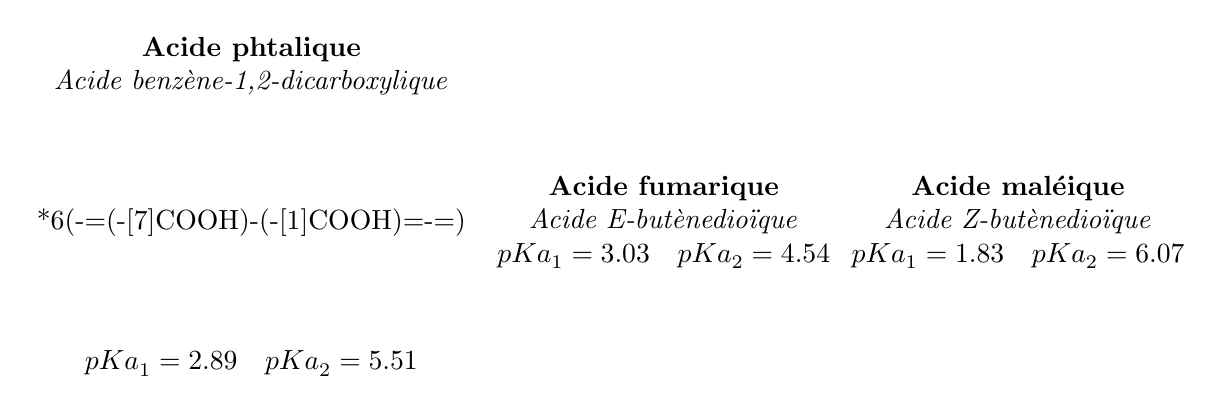
\begin{tikzpicture}
    \draw (0,0) 
        node{
    \chemfig{*6(-=(-[7]COOH)-(-[1]COOH)=-=)}
    } 
        node[above=1.5cm, align=center]{\textbf{Acide phtalique}\\ \textit{Acide benzène-1,2-dicarboxylique}}
        
        node[below=1.5cm]{$\text{pKa}_1=2.89$\quad $\text{pKa}_2=5.51$}
        
        node[right=3cm, align=center] {\textbf{Acide fumarique}\\\textit{Acide E-butènedioïque}\\ $\text{pKa}_1=3.03$\quad $\text{pKa}_2=4.54$}
        
        node[right=7.5cm, align=center] {\textbf{Acide maléique}\\\textit{Acide Z-butènedioïque}\\ $\text{pKa}_1=1.83$\quad $\text{pKa}_2=6.07$};
        
\end{tikzpicture}
\end{minipage}\\

\begin{itemize}
    \item Comparer les pKa de l’acide maléique, fumarique et phtalique 
    \item Réaction avec une molécule comportant un cycle dans une solution tampon de $pH = 7.5$, qui ne pouvait se faire que sur le carbone R de la molécule (mon souvenir est flou étant donné que je n’ai pas traité cette question)
    \item Titrage des acides
\end{itemize}

\hrulefill\\

Seul l’acide phtalique était donné dans le sujet, j’ai donc représenté les deux autres molécules que je connaissais (je crois qu’il y avait les noms développés au cas où).\\

\begin{center}
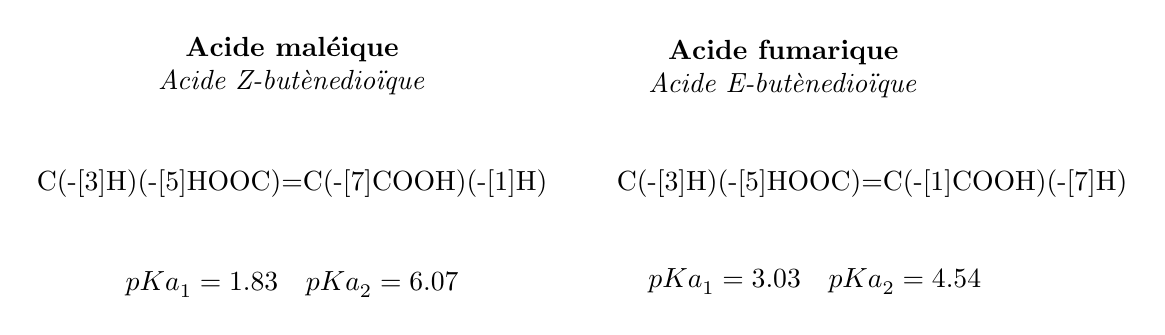
\begin{tikzpicture}
    \draw (0,0) 
    
    node{
    \chemfig{C(-[3]H)(-[5]HOOC)=C(-[7]COOH)(-[1]H)}
    }
    
    node
    [above=1cm, align=center]
    {
    \textbf{Acide maléique}\\\textit{Acide Z-butènedioïque}
    }
    
    node
    [below=1cm]
    {
    $\text{pKa}_1=1.83$\quad $\text{pKa}_2=6.07$
    }
    
    node
    [right=4cm]
    {
    \chemfig{C(-[3]H)(-[5]HOOC)=C(-[1]COOH)(-[7]H)}
    }
    
    node
    [right=4.4cm, yshift=1.45cm, align=center]
    {
    \textbf{Acide fumarique}\\\textit{Acide E-butènedioïque}
    }
    
    node
    [right=4.4cm, yshift=-1.25cm]
    {
    $\text{pKa}_1=3.03$\quad $\text{pKa}_2=4.54$
    };
\end{tikzpicture}
\end{center}

J’ai essayé de mobiliser plusieurs arguments pour justifier les différences de pKa : l’isomérie Z/E, la présence de liaisons hydrogènes intramoléculaires (pour cela, il faut représenter les liaisons développées avec les doublets), les différentes formes mésomères.

\begin{center}
    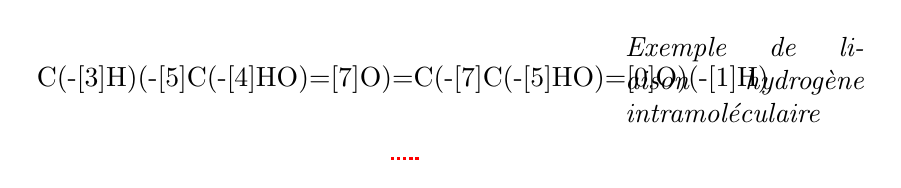
\begin{tikzpicture}
        \draw (0,0) node{
        \chemfig{C(-[3]H)(-[5]C(-[4]HO)=[7]O)=C(-[7]C(-[5]HO)=[0]O)(-[1]H)}
        }
        node[right=2.7cm]{
        \begin{minipage}{0.25\linewidth}
            \textit{Exemple de liaison hydrogène intramoléculaire}
        \end{minipage}
        };
        \draw[densely dotted, very thick, color=red] (-.15,-1)--++(.35,0);
    \end{tikzpicture}
\end{center}
L’examinateur me posait pas mal de questions assez détaillées, sûrement parce que j’étalais tout mon raisonnement interne (et donc mes hésitations) à l’oral. Ces questions interrogeaient ma conception de chaque grandeur ou phénomène abordé (définition du pKa, d’un mésomère attracteur/donneur, énergie des différentes liaisons). \\
Je vous conseille d’être vraiment à l’aise sur ces concepts de base en chimie, parce que même si on les comprend en PASS, devoir les expliquer clairement et avec les bons mots c’est autre chose. Par exemple, l’examinateur est revenu sur mes mots lorsque j’ai dit « la molécule lâche plus vite son proton » en me demandant si le pKa était une constante de vitesse, ce à quoi j’ai répondu non (en essayant de contrôler mes mots ensuite) puis ai défini le pKa.\\ 
Il ne restait que quelques minutes et l’examinateur m’a demandé de traiter la troisième question. Je n’ai donc pu que communiquer un raisonnement à l’oral et mes intuitions, mais il paraissait plutôt satisfait finalement. \\
Au cours de l’oral l’examinateur vous guide bien et pose souvent des questions du tac au tac, et n’hésitez pas à montrer que vous êtes intéressés en posant des questions par exemple (mais n’en posez pas pour en poser). \\

\lettrine{{\color{violet} \oldpilcrowfive}}{}
Le texte qui suit est la remise en page de la photo que tu pourras retrouver \href{https://drive.google.com/file/d/1OXCKLgBEOjYLlkHNkYJIklnAarVVDgL3/view?usp=sharing}{<ici>}\footnote{https://drive.google.com/file/d/1OXCKLgBEOjYLlkHNkYJIklnAarVVDgL3/view?usp=sharing}.\\

$$
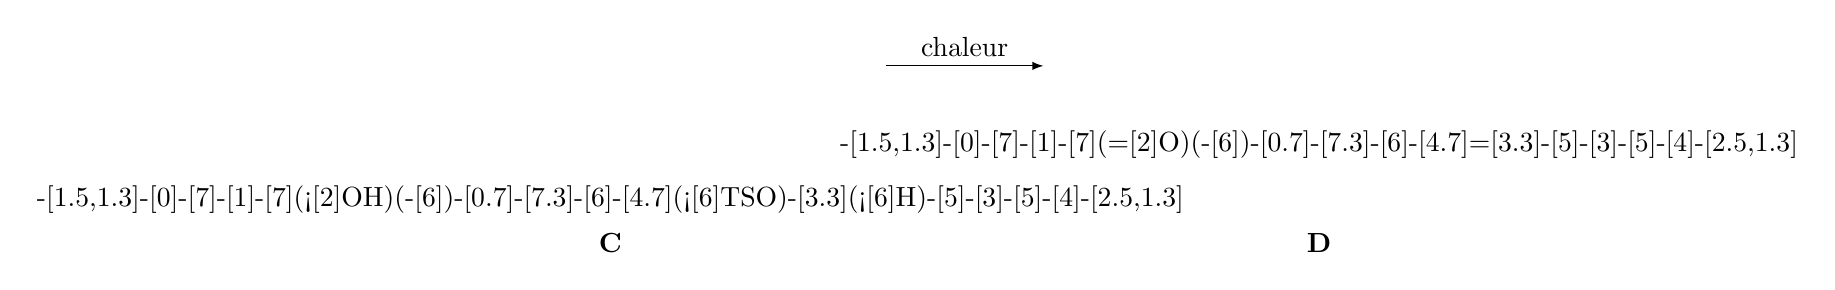
\begin{tikzpicture}
\draw (0,0) node[above]{
\chemfig{-[1.5,1.3]-[0]-[7]-[1]-[7](<[2]OH)(-[6])-[0.7]-[7.3]-[6]-[4.7](<[6]TSO)-[3.3](<[6]H)-[5]-[3]-[5]-[4]-[2.5,1.3]}
};
\draw (0,0) node[below]{\textbf{C}};

\draw[->,>=latex](3.5,2)--++(2,0) node[midway,above]{chaleur};

\draw (9,0) node[above=0.7cm] {
\chemfig{-[1.5,1.3]-[0]-[7]-[1]-[7](=[2]O)(-[6])-[0.7]-[7.3]-[6]-[4.7]=[3.3]-[5]-[3]-[5]-[4]-[2.5,1.3]}
};
\draw (9,0) node[below]{\textbf{D}};
\end{tikzpicture}
$$


\begin{enumerate}[label=\alph*)]
    \item Ecrire le mécanisme réactionnel de \textbf{C} avec le tert-butanolate de potassium pour obtenir \textbf{D}.
    \item Quelles réactions parasites peuvent se produire ? Pourquoi cela n'est pas le cas ?
\end{enumerate}
\newpage
